\documentclass[tikz,border=3pt]{standalone}
\usetikzlibrary{arrows.meta}

\definecolor{textcolor}{HTML}{0F172A}
\definecolor{muted}{HTML}{475569}
\definecolor{panel}{HTML}{F8FAFC}
\definecolor{edgecolor}{HTML}{334155}
\definecolor{softcyan}{HTML}{E0F2FE}
\definecolor{cyanedge}{HTML}{0E7490}
\definecolor{softblue}{HTML}{DBEAFE}
\definecolor{blueedge}{HTML}{2563EB}
\definecolor{softgreen}{HTML}{DCFCE7}
\definecolor{greenedge}{HTML}{16A34A}
\definecolor{softorange}{HTML}{FFEDD5}
\definecolor{orangeedge}{HTML}{EA580C}
\definecolor{softrose}{HTML}{FFE4E6}
\definecolor{roseedge}{HTML}{E11D48}
\definecolor{softviolet}{HTML}{EDE9FE}
\definecolor{violetedge}{HTML}{7C3AED}

\tikzset{
  box/.style={
    rounded corners=2pt,
    align=center,
    draw=edgecolor,
    line width=0.45pt,
    inner sep=4pt,
    font=\sffamily\scriptsize,
    text=textcolor
  },
  input/.style={box, fill=softcyan, draw=cyanedge, minimum width=2.55cm, minimum height=0.86cm},
  backbone/.style={box, fill=softblue, draw=blueedge, minimum width=2.65cm, minimum height=0.92cm},
  adapter/.style={box, fill=softgreen, draw=greenedge, minimum width=2.65cm, minimum height=0.86cm},
  train/.style={box, fill=softorange, draw=orangeedge, minimum width=2.75cm, minimum height=0.72cm},
  dag/.style={box, fill=softviolet, draw=violetedge, minimum width=2.75cm, minimum height=0.72cm},
  output/.style={box, fill=softrose, draw=roseedge, minimum width=2.45cm, minimum height=0.86cm},
  edge/.style={-Latex, draw=edgecolor, line width=0.58pt},
  control/.style={-Latex, draw=greenedge, line width=0.64pt},
  trainflow/.style={-Latex, draw=orangeedge, dashed, line width=0.50pt},
  note/.style={font=\sffamily\tiny, text=muted}
}

\begin{document}
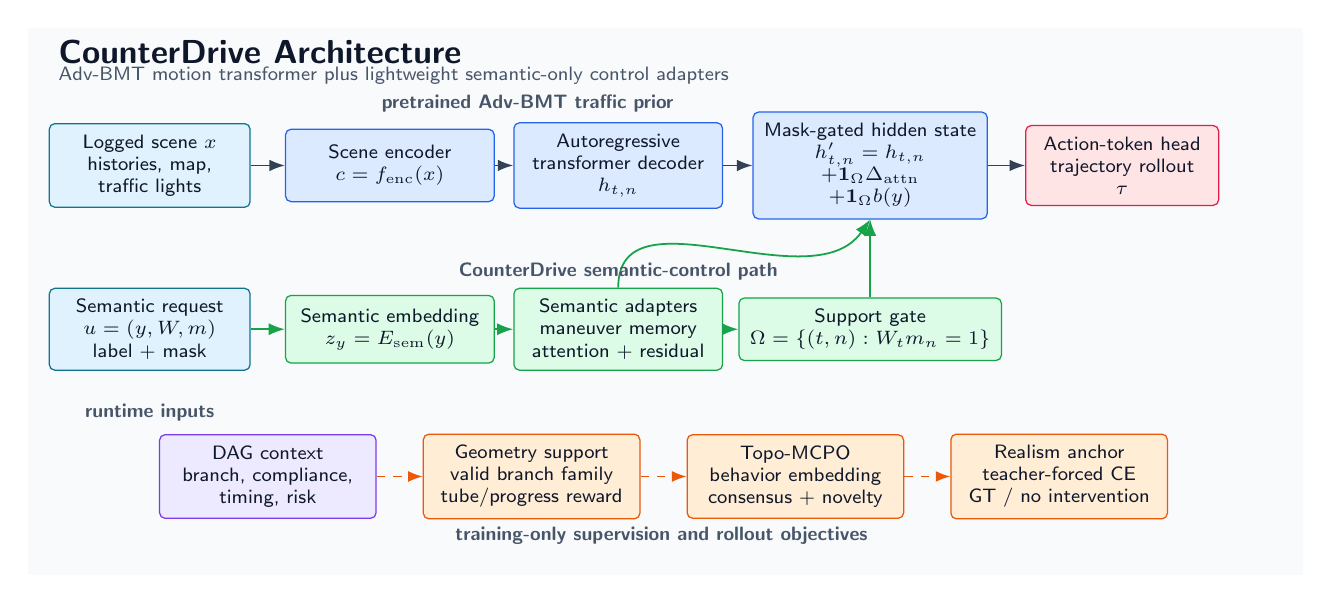
\begin{tikzpicture}[x=1cm,y=1cm]
  \fill[panel] (-0.35,-0.30) rectangle (15.85,6.65);

  \node[anchor=west, font=\sffamily\bfseries\large, text=textcolor] at (-0.08,6.34)
    {CounterDrive Architecture};
  \node[anchor=west, font=\sffamily\scriptsize, text=muted] at (-0.08,6.04)
    {Adv-BMT motion transformer plus lightweight semantic-only control adapters};

  % Runtime inputs.
  \node[input] (scene) at (1.20,4.90)
    {Logged scene $x$\\ histories, map,\\ traffic lights};
  \node[input] (request) at (1.20,2.82)
    {Semantic request\\ $u=(y,W,m)$\\ label + mask};

  % Backbone path.
  \node[backbone] (encoder) at (4.25,4.90)
    {Scene encoder\\ $c=f_{\rm enc}(x)$};
  \node[backbone] (decoder) at (7.15,4.90)
    {Autoregressive\\ transformer decoder\\ $h_{t,n}$};
  \node[backbone] (controlled) at (10.35,4.90)
    {Mask-gated hidden state\\
    $h'_{t,n}=h_{t,n}$\\
    $+\mathbf{1}_{\Omega}\Delta_{\rm attn}$\\
    $+\mathbf{1}_{\Omega}b(y)$};
  \node[output] (head) at (13.55,4.90)
    {Action-token head\\ trajectory rollout\\ $\tau$};

  % Semantic-control path.
  \node[adapter] (embed) at (4.25,2.82)
    {Semantic embedding\\ $z_y=E_{\rm sem}(y)$};
  \node[adapter] (adapters) at (7.15,2.82)
    {Semantic adapters\\ maneuver memory\\ attention + residual};
  \node[adapter, minimum width=2.20cm, minimum height=0.68cm] (gate) at (10.35,2.82)
    {Support gate\\ $\Omega=\{(t,n):W_t m_n=1\}$};

  % Training-only blocks.
  \node[dag] (dagctx) at (2.70,0.95)
    {DAG context\\ branch, compliance,\\ timing, risk};
  \node[train] (family) at (6.05,0.95)
    {Geometry support\\ valid branch family\\ tube/progress reward};
  \node[train] (topo) at (9.40,0.95)
    {Topo-MCPO\\ behavior embedding\\ consensus + novelty};
  \node[train] (ce) at (12.75,0.95)
    {Realism anchor\\ teacher-forced CE\\ GT / no intervention};

  % Runtime arrows.
  \draw[edge] (scene.east) -- (encoder.west);
  \draw[edge] (encoder.east) -- (decoder.west);
  \draw[edge] (decoder.east) -- (controlled.west);
  \draw[edge] (controlled.east) -- (head.west);

  \draw[control] (request.east) -- (embed.west);
  \draw[control] (embed.east) -- (adapters.west);
  \draw[control] (adapters.east) -- (gate.west);
  \draw[control] (adapters.north) to[out=90,in=235] (controlled.south);
  \draw[control] (gate.north) -- (controlled.south);

  % Training arrows.
  \draw[trainflow] (dagctx.east) -- (family.west);
  \draw[trainflow] (family.east) -- (topo.west);
  \draw[trainflow] (topo.east) -- (ce.west);

  % Labels.
  \node[font=\sffamily\scriptsize\bfseries, text=muted] at (1.20,1.76) {runtime inputs};
  \node[font=\sffamily\scriptsize\bfseries, text=muted] at (6.00,5.68) {pretrained Adv-BMT traffic prior};
  \node[font=\sffamily\scriptsize\bfseries, text=muted] at (7.15,3.55) {CounterDrive semantic-control path};
  \node[font=\sffamily\scriptsize\bfseries, text=muted] at (7.70,0.20) {training-only supervision and rollout objectives};

\end{tikzpicture}
\end{document}
